\documentclass{letter}
\usepackage{hyperref}
\usepackage{graphicx}
\usepackage{color}

\signature{Patrick Sanan}
\address{Dienerstrasse 15\\ Z\"{u}rich 8004\\ Switzerland}
\begin{document}
\begin{letter}{Stephanie Frequente\\CSCS Human Resources\\via Trevano 131\\6900 Lugano\\Switzerland}
\opening{Dear Ms. Frequente,}

I am writing to apply for the position of Scientific Software Developer.

I believe that I am a strong candidate as I have broad experience in computational mathematics and computational science; I have a PhD in applied/computational mathematics, have worked extensively with both library and application codes as part of my current job as a postdoc on a PASC project, am a native English speaker, and have experience using CSCS's systems.

I am very interested in the collaborative aspect of this position, and would hope to be paired with teams working on topics I have touched on before, such as geophysics, communication-hiding algorithms, or numerical methods. In particular, I would be excited to work with a team leveraging the PETSc library, to which I am eager to contribute as a developer.

To me, ``Modern C++'' means a set of tools which are often fun, occasionally elegant, and usually overkill. Especially in scientific computing, much of what we need to do can (and is) accomplished in C or Fortran, so my personal preference with C++ is to favor less-elaborate designs which are more easily comprehended, debugged, profiled, and transferred to new developers. Extremely clever inheritance trees, template metaprogramming, etc., should not be introduced without very clear justification. 

\closing{Sincerely,}
%\hfill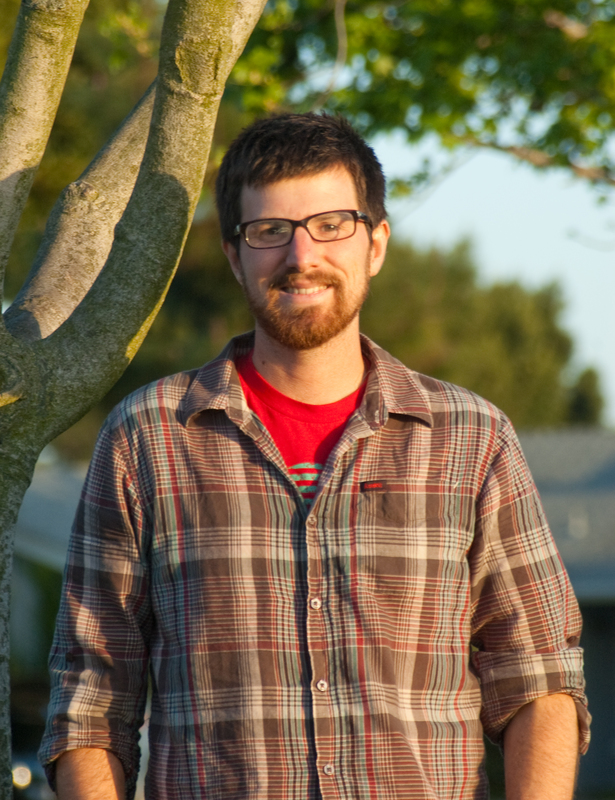
\includegraphics[width=170px]{sanan_patrick_portrait_small.jpg}
\end{letter}

\end{document}
